\documentclass[10pt,a4paper]{article}
\usepackage[margin=2.2cm,top=2.4cm,headsep=0.5cm]{geometry}
\usepackage[T1]{fontenc}
\usepackage{lmodern}
\usepackage[scaled=0.94]{helvet}
\renewcommand{\familydefault}{\sfdefault}
\usepackage{microtype}
\usepackage[parfill]{parskip}
\usepackage{fancyhdr}
\usepackage{titlesec}
\usepackage{amsmath,amssymb}
\usepackage{graphicx}
\usepackage{booktabs}
\usepackage{array}
\usepackage{caption}
\usepackage{algorithm}
\usepackage{algpseudocode}
\usepackage[dvipsnames]{xcolor}
\usepackage{listings}
\usepackage[colorlinks=true,linkcolor=MidnightBlue,citecolor=MidnightBlue,urlcolor=MidnightBlue]{hyperref}
\usepackage[nameinlink]{cleveref}

\graphicspath{{../figures/}}
% generated by scripts/make_plots.py -- do not edit
\newcommand{\CGbwAll}{1395}
\newcommand{\CGbwEight}{136}
\newcommand{\CGbwFrac}{77}
\newcommand{\CGbwFracNodes}{81}
\newcommand{\CGbwFracStreamNodes}{62}
\newcommand{\CGbwNode}{215}
\newcommand{\CGbwOne}{23.9}
\newcommand{\CGbwPerNodeMax}{174}
\newcommand{\CGbwSixteen}{183}
\newcommand{\CGbwTB}{1.40}
\newcommand{\CVN}{256}
\newcommand{\CVP}{64}
\newcommand{\CVmsgsOneD}{2}
\newcommand{\CVmsgsThreeD}{6}
\newcommand{\CVoneD}{1.00}
\newcommand{\CVratio}{5.3}
\newcommand{\CVthreeD}{0.19}
\newcommand{\CommFracNode}{5}
\newcommand{\CommFracPmax}{28}
\newcommand{\ConvTwoNmax}{256}
\newcommand{\ConvTwoNmin}{32}
\newcommand{\DriftCG}{$6\times10^{-13}$}
\newcommand{\DriftPipe}{$7\times10^{-8}$}
\newcommand{\EffFour}{98}
\newcommand{\EffNode}{28}
\newcommand{\EffPmax}{23}
\newcommand{\FinalCG}{$6\times10^{-13}$}
\newcommand{\FinalPipe}{$4\times10^{-9}$}
\newcommand{\FloorCG}{$6\times10^{-13}$}
\newcommand{\FloorPipe}{$1\times10^{-11}$}
\newcommand{\FloorRatio}{15}
\newcommand{\GpuBwAboveMin}{454}
\newcommand{\GpuBwFiveTwelve}{473}
\newcommand{\GpuBwFrac}{68}
\newcommand{\GpuBwMax}{474}
\newcommand{\GpuBwMin}{416}
\newcommand{\GpuBwRatio}{2.2}
\newcommand{\GpuCGoneRel}{2}
\newcommand{\GpuDofsMax}{453}
\newcommand{\GpuDriver}{575.57.08}
\newcommand{\GpuMLUPS}{5.37}
\newcommand{\GpuMem}{45\,GiB usable}
\newcommand{\GpuModule}{nvhpc-hpcx-cuda12/26.1}
\newcommand{\GpuNVC}{26.1-0}
\newcommand{\GpuName}{NVIDIA A40}
\newcommand{\GpuNmax}{768}
\newcommand{\GpuNmin}{128}
\newcommand{\GpuSpmvBw}{276}
\newcommand{\GpuSpmvBwFrac}{40}
\newcommand{\GpuSpmvFrac}{31}
\newcommand{\GpuTfiveTwelve}{25.0}
\newcommand{\GpuTwoBw}{477}
\newcommand{\GpuTwoBwMax}{494}
\newcommand{\GpuTwoBwMin}{388}
\newcommand{\GpuTwoDofsMax}{268}
\newcommand{\GpuTwoN}{8192}
\newcommand{\GpuTwoNmax}{16384}
\newcommand{\GpuTwoNmin}{1024}
\newcommand{\GpuTwoSolve}{322}
\newcommand{\GpuTwoSpmvBw}{322}
\newcommand{\GpuTwoT}{12.37}
\newcommand{\GpuTwoVecBw}{535}
\newcommand{\GpuTwoVsEight}{2.7}
\newcommand{\GpuTwoVsSocket}{2.7}
\newcommand{\GpuValFail}{0}
\newcommand{\GpuValP}{1, 2, 4, 8}
\newcommand{\GpuValRuns}{8}
\newcommand{\GpuValTwoFail}{0}
\newcommand{\GpuValTwoP}{1, 2, 4}
\newcommand{\GpuValTwoRuns}{6}
\newcommand{\GpuValTwoWorst}{$7.4\times10^{-15}$}
\newcommand{\GpuValWorst}{$4.0\times10^{-15}$}
\newcommand{\GpuVecBw}{562}
\newcommand{\GpuVecBwFrac}{81}
\newcommand{\GpuVsCore}{22}
\newcommand{\GpuVsEight}{2.7}
\newcommand{\GpuVsSocket}{2.4}
\newcommand{\HaloFracPmax}{6}
\newcommand{\HaloKiBNode}{1152}
\newcommand{\HaloKiBPmax}{320}
\newcommand{\HaloMsPmax}{0.52}
\newcommand{\HybBest}{32$\times$8}
\newcommand{\HybBestT}{8.72}
\newcommand{\HybCores}{256}
\newcommand{\HybGain}{6}
\newcommand{\HybPureT}{9.23}
\newcommand{\HybRange}{9}
\newcommand{\HybRedBest}{1.51}
\newcommand{\HybRedPure}{2.07}
\newcommand{\HybSecond}{64$\times$4}
\newcommand{\HybSecondT}{9.45}
\newcommand{\HybWorst}{8$\times$32}
\newcommand{\HybWorstT}{9.46}
\newcommand{\Iters}{50}
\newcommand{\LastCG}{365}
\newcommand{\LastPipe}{700}
\newcommand{\MachineCPN}{32}
\newcommand{\MachineCPS}{36}
\newcommand{\MachineCPU}{Intel Xeon Platinum 8452Y}
\newcommand{\MachineCores}{256}
\newcommand{\MachineGCC}{13.1.0}
\newcommand{\MachineMPI}{Open MPI 4.1.8}
\newcommand{\MachineNodes}{8}
\newcommand{\MaxSpread}{166}
\newcommand{\MedSpread}{3.7}
\newcommand{\NS}{512}
\newcommand{\NSdofs}{134}
\newcommand{\NStwo}{768}
\newcommand{\NStwoDofs}{453}
\newcommand{\NodeCPU}{Intel Xeon Platinum 8452Y}
\newcommand{\NodeEffPmax}{81}
\newcommand{\NodeEffSixtyFour}{83}
\newcommand{\NodeEffTwoPmax}{83}
\newcommand{\NodeSpeedPmax}{6.50}
\newcommand{\NodeSpeedTwoPmax}{6.60}
\newcommand{\NodeValCG}{$3.8\times10^{-15}$}
\newcommand{\NodeValEdge}{12}
\newcommand{\NodeValPipe}{$2.0\times10^{-12}$}
\newcommand{\NodeValResult}{passes}
\newcommand{\NodeValRuns}{36}
\newcommand{\NodesMax}{8}
\newcommand{\OrderMax}{2.000}
\newcommand{\OrderMin}{1.999}
\newcommand{\OrderTwoMax}{2.000}
\newcommand{\OrderTwoMin}{2.000}
\newcommand{\Pmax}{256}
\newcommand{\PoneFaster}{faster}
\newcommand{\PoneTiter}{540}
\newcommand{\PoneVsSerial}{1.2}
\newcommand{\RedFracPmax}{22}
\newcommand{\RedMsNode}{1.04}
\newcommand{\RedMsPmax}{2.07}
\newcommand{\RelBlocking}{0.98}
\newcommand{\RelBlockingRange}{0.96--1.01}
\newcommand{\RelCGone}{1.02}
\newcommand{\RelCGoneRange}{0.97--1.02}
\newcommand{\RelCGonemin}{1.01}
\newcommand{\RelOneD}{1.65}
\newcommand{\RelOneDmin}{1.14}
\newcommand{\RelPipe}{1.24}
\newcommand{\RelPipeBlock}{1.26}
\newcommand{\RelPipeTwo}{1.28}
\newcommand{\RelPipemin}{1.32}
\newcommand{\RelTwoD}{1.14}
\newcommand{\RelTwoDRange}{0.95--1.14}
\newcommand{\Reps}{3}
\newcommand{\SerialTiter}{546}
\newcommand{\SizesCPU}{Intel Xeon Platinum 8452Y}
\newcommand{\SolveCG}{21.0}
\newcommand{\SolveCGTrue}{$9.8\times10^{-9}$}
\newcommand{\SolveCGone}{20.6}
\newcommand{\SolveGpu}{48.5}
\newcommand{\SolveGpuIters}{1942}
\newcommand{\SolveGpuSpeedup}{22}
\newcommand{\SolveIters}{1942}
\newcommand{\SolvePipe}{25.5}
\newcommand{\SolvePipeRatio}{70}
\newcommand{\SolvePipeTrue}{$7.0\times10^{-7}$}
\newcommand{\SolveSerialEst}{1061}
\newcommand{\SolveSerialMeas}{1187}
\newcommand{\SolveSpeedup}{50}
\newcommand{\SpeedupEight}{5.8}
\newcommand{\SpeedupFour}{3.91}
\newcommand{\SpeedupNode}{9.1}
\newcommand{\SpeedupPmax}{59.2}
\newcommand{\SplitCG}{$3\times10^{-13}$}
\newcommand{\SplitPipe}{$9\times10^{-11}$}
\newcommand{\StreamAll}{279}
\newcommand{\StreamEight}{131}
\newcommand{\StreamOne}{20.0}
\newcommand{\StreamSixteen}{192}
\newcommand{\StreamThreads}{32}
\newcommand{\SzBwLarge}{21.1}
\newcommand{\SzBwMax}{30}
\newcommand{\SzBwMin}{17}
\newcommand{\SzDofsMax}{134}
\newcommand{\SzDoubling}{14.5}
\newcommand{\SzGiBLarge}{4.0}
\newcommand{\SzItMax}{1942}
\newcommand{\SzItMin}{235}
\newcommand{\SzItPerN}{3.79}
\newcommand{\SzItPerNmax}{3.79}
\newcommand{\SzItPerNmin}{3.67}
\newcommand{\SzMiBSmall}{8.8}
\newcommand{\SzNmax}{512}
\newcommand{\SzNmin}{64}
\newcommand{\SzNsLarge}{4.55}
\newcommand{\SzNsMax}{5.62}
\newcommand{\SzNsMin}{3.21}
\newcommand{\SzNsSmall}{4.13}
\newcommand{\SzNsolveMax}{512}
\newcommand{\SzSlopeIter}{3.03}
\newcommand{\SzSlopeSolve}{4.05}
\newcommand{\SzSolveMax}{1187}
\newcommand{\SzSolveMaxMin}{19.8}
\newcommand{\SzSolveMin}{0.25}
\newcommand{\SzTiterMax}{611}
\newcommand{\SzTwoBwLarge}{24.7}
\newcommand{\SzTwoBwMax}{55}
\newcommand{\SzTwoBwMin}{25}
\newcommand{\SzTwoDofsMax}{67}
\newcommand{\SzTwoDoubling}{8.4}
\newcommand{\SzTwoGiBLarge}{6.0}
\newcommand{\SzTwoItMax}{12884}
\newcommand{\SzTwoItMin}{771}
\newcommand{\SzTwoItPerN}{3.15}
\newcommand{\SzTwoItPerNmax}{3.15}
\newcommand{\SzTwoItPerNmin}{3.01}
\newcommand{\SzTwoMiBSmall}{6.1}
\newcommand{\SzTwoNmax}{8192}
\newcommand{\SzTwoNmin}{256}
\newcommand{\SzTwoNsLarge}{3.89}
\newcommand{\SzTwoNsMax}{3.89}
\newcommand{\SzTwoNsMin}{1.74}
\newcommand{\SzTwoNsSecond}{2.65}
\newcommand{\SzTwoNsSmall}{1.74}
\newcommand{\SzTwoNsecond}{512}
\newcommand{\SzTwoNsolveMax}{4096}
\newcommand{\SzTwoSlopeIter}{2.22}
\newcommand{\SzTwoSlopeSolve}{3.27}
\newcommand{\SzTwoSolveMax}{781}
\newcommand{\SzTwoSolveMaxMin}{13.0}
\newcommand{\SzTwoSolveMin}{0.09}
\newcommand{\SzTwoTiterMax}{261}
\newcommand{\TiterNode}{60.1}
\newcommand{\TiterPmax}{9.23}
\newcommand{\TiterSixtyFour}{36.0}
\newcommand{\TiterTwoNode}{201.6}
\newcommand{\TiterTwoPmax}{30.5}
\newcommand{\TwoBlockMax}{0.95}
\newcommand{\TwoBlockRange}{0.95--1.05}
\newcommand{\TwoBwMax}{1412}
\newcommand{\TwoBwNode}{195}
\newcommand{\TwoCGoneMax}{0.93}
\newcommand{\TwoCGoneRange}{0.92--1.01}
\newcommand{\TwoCommMax}{35}
\newcommand{\TwoDofs}{67}
\newcommand{\TwoEffMax}{19}
\newcommand{\TwoEffNode}{22}
\newcommand{\TwoHaloFracMax}{5}
\newcommand{\TwoHaloKiBMax}{16}
\newcommand{\TwoHaloMsMax}{0.22}
\newcommand{\TwoLocalMax}{512$\times$512}
\newcommand{\TwoMsgsMax}{4}
\newcommand{\TwoN}{8192}
\newcommand{\TwoNodeEffMax}{90}
\newcommand{\TwoNodeSpeedMax}{7.23}
\newcommand{\TwoPoneT}{228}
\newcommand{\TwoRedFracMax}{30}
\newcommand{\TwoRedMsMax}{1.39}
\newcommand{\TwoSlabBest}{0.82}
\newcommand{\TwoSlabHaloKiB}{128}
\newcommand{\TwoSlabMax}{0.82}
\newcommand{\TwoSlabMin}{0.97}
\newcommand{\TwoSlabPct}{18}
\newcommand{\TwoSolveCG}{135}
\newcommand{\TwoSolveCGone}{126}
\newcommand{\TwoSolveCGoneGain}{7}
\newcommand{\TwoSolveIters}{26046}
\newcommand{\TwoSolveSerialEst}{5930}
\newcommand{\TwoSolveSpeedup}{44}
\newcommand{\TwoSolveTrue}{$8.2\times10^{-8}$}
\newcommand{\TwoSpeedFour}{3.28}
\newcommand{\TwoSpeedMax}{49.9}
\newcommand{\TwoSpeedNode}{6.9}
\newcommand{\TwoTmax}{4.56}
\newcommand{\TwoTnode}{33.0}
\newcommand{\TwoWeakDofsMax}{1.07}
\newcommand{\TwoWeakEffNode}{27}
\newcommand{\TwoWeakLocal}{2048}
\newcommand{\TwoWeakNmax}{32768}
\newcommand{\TwoWeakNodeEff}{93}
\newcommand{\TwoWeakTmax}{70.0}
\newcommand{\TwoWeakTnode}{65.4}
\newcommand{\TwoWeakTone}{17.5}
\newcommand{\ValEdge}{30}
\newcommand{\ValErrMax}{$2.39\times10^{-5}$}
\newcommand{\ValIters}{146}
\newcommand{\ValN}{40}
\newcommand{\ValRuns}{180}
\newcommand{\ValTwoEdge}{30}
\newcommand{\ValTwoErrMax}{$9.12\times10^{-6}$}
\newcommand{\ValTwoIters}{298}
\newcommand{\ValTwoRuns}{120}
\newcommand{\ValTwoWorstCG}{$6.9\times10^{-15}$}
\newcommand{\ValTwoWorstPipe}{$3.1\times10^{-11}$}
\newcommand{\ValWorstCG}{$3.8\times10^{-15}$}
\newcommand{\ValWorstPipe}{$2.0\times10^{-12}$}
\newcommand{\VarP}{256}
\newcommand{\VarPmin}{32}
\newcommand{\VecFracSerial}{56}
\newcommand{\WeakBwNode}{6.8}
\newcommand{\WeakBwOne}{18.1}
\newcommand{\WeakDofsMax}{1.81}
\newcommand{\WeakEffNode}{38}
\newcommand{\WeakEffPmax}{30}
\newcommand{\WeakLocal}{192}
\newcommand{\WeakNmax}{1219}
\newcommand{\WeakNodeEff}{80}
\newcommand{\WeakPmax}{256}
\newcommand{\WeakTmax}{125.1}
\newcommand{\WeakTmidMax}{121}
\newcommand{\WeakTmidMin}{119}
\newcommand{\WeakTnode}{100.5}
\newcommand{\WeakTone}{37.4}
\newcommand{\WeakTtwo}{119.1}


% \input inside a tabular breaks \bottomrule; the TeX primitive does not
\makeatletter\newcommand{\tabinput}[1]{\@@input #1 }\makeatother
\captionsetup{font=normalsize,labelfont=normalfont,labelsep=colon,skip=6pt}
\titleformat{\section}{\large\bfseries}{\thesection.}{0.5em}{}
\titleformat{\subsection}{\normalsize\bfseries}{\thesubsection}{0.6em}{}
\titlespacing*{\section}{0pt}{14pt}{6pt}
\titlespacing*{\subsection}{0pt}{10pt}{4pt}
\pagestyle{fancy}\fancyhf{}
\fancyhead[L]{\small DSA5208 \textbar{} Parallel Conjugate Gradients}
\fancyhead[R]{\small MPI\,+\,OpenMP on NUS Vanda}
\fancyfoot[C]{\small\thepage}
\renewcommand{\headrulewidth}{0.4pt}
\lstset{basicstyle=\ttfamily\small,columns=fullflexible,keepspaces=true,frame=single,
        framerule=0.3pt,rulecolor=\color{gray!60},backgroundcolor=\color{gray!4}}
\newcommand{\code}[1]{\texttt{#1}}
\newcommand{\vb}[1]{\mathbf{#1}}
\emergencystretch=2em

\begin{document}
\thispagestyle{plain}
\begin{center}
{\LARGE\bfseries Scaling Conjugate Gradients with MPI and OpenMP\par}
\vspace{4pt}
{\large Decomposition, communication hiding, memory bandwidth and GPU offload in matrix-free 2D and 3D Poisson solvers\par}
\vspace{10pt}
\begin{tabular*}{\linewidth}{@{\extracolsep{\fill}}ccc}
WU YUHAN (A0351706H) & ZUO DEWEI (A0352507H) & ZHU CHEN (A0357394N)
\end{tabular*}\par
\vspace{6pt}
DSA5208 $\cdot$ Project 3\par
\end{center}
\vspace{4pt}

\noindent{\large\bfseries Abstract}\par
\noindent
The Conjugate Gradient (CG) method is the standard solver for the symmetric positive definite systems
produced by elliptic partial differential equations, and it is hard to scale: every iteration
needs a nearest-neighbour exchange, two global reductions and a full sweep through memory. We build a
matrix-free CG solver for the 2D and 3D Poisson equation in three versions---serial, hybrid MPI\,+\,OpenMP, and
MPI\,+\,OpenMP target offload to GPUs---in which domain decomposition, halo exchange, reduction strategy and
the split between processes and threads are run-time switches, and measure each choice on the NUS Vanda
cluster from one core to \Pmax{} cores on \NodesMax{} nodes and on an NVIDIA A40. In \ValRuns{} CPU and
\GpuValRuns{} GPU configurations the solvers reproduce the serial solution to rounding level (\ValWorstCG{}
for classic CG and CG1, \ValWorstPipe{} for pipelined CG), and they converge at the theoretical second
order. Inside a socket CG scales exactly as far as memory bandwidth does: 32 cores
reach a speedup of \SpeedupNode{} and \CGbwFrac\% of the STREAM bandwidth. Across nodes every socket
brings its own memory, and \Pmax{} cores run a $512^3$ iteration in \TiterPmax\,ms, a speedup of
\SpeedupPmax{} with \NodeEffPmax\% efficiency relative to one node (\NodeEffTwoPmax\% for $768^3$) and
\WeakNodeEff\% weak-scaling efficiency on 1.8 billion unknowns. At that scale the global reductions, not the
halo messages, cost most: they take \RedFracPmax\% of an iteration against \HaloFracPmax\% for the halo
exchange, almost all of it waiting at a barrier. Neither merging the two reductions nor pipelining them
removes that wait. The 2D problem confirms both mechanisms and reverses one design choice: its halo is a
\TwoHaloKiBMax\,KiB trickle, \Pmax{} cores reach \TwoNodeEffMax\% strong and \TwoWeakNodeEff\% weak
efficiency relative to one node, and slabs, which lose a factor \RelOneD{} in 3D, take \TwoSlabPct\%
less time than blocks in 2D. One A40 runs an iteration \GpuVsSocket{} (3D) and \GpuTwoVsSocket{} (2D) times
faster than a 32-core CPU socket.

\section{Introduction}\label{sec:intro}

Many simulation codes spend most of their run time solving a single kind of linear system. The pressure
projection of incompressible flow solvers, the electrostatic potential in plasma and molecular dynamics,
the gravitational potential in astrophysics and graph-Laplacian systems in semi-supervised learning and
spectral clustering all reduce to a Poisson-type equation that has to be solved again at every time step
or outer iteration. Discretising $-\nabla^2u=f$ on a cube with $N$ grid points per direction yields
$N^3$ unknowns, and refining the grid makes the problem harder twice over: the system grows like $N^3$,
and the number of iterations of a Krylov solver grows like $N$, so the total work grows like $N^4$. A
$512^3$ grid already holds 134 million unknowns, needs about two thousand CG iterations and takes
\SzSolveMaxMin{} minutes on one core. Solving such problems in reasonable time and memory requires
distributing them across many nodes.

The Conjugate Gradient method is the method of choice for these symmetric positive definite systems, and
it is also a standard stress test for parallel computers: the HPCG benchmark~[4], which complements LINPACK
in the TOP500 ranking, is built around it because supercomputers reach only a few percent of their peak
performance on it. The reason lies in the structure of a single iteration. Its matrix--vector product
couples every unknown to its grid neighbours, so a distributed implementation has to exchange the
boundary layers (\emph{halos}) of every subdomain in every iteration. Its two inner products couple every
unknown to every other one; each requires a global reduction that acts as a barrier across all
processes and whose latency grows with the number of processes $P$. Since every iteration needs the
scalars produced by the previous one, none of this communication can be batched or deferred across
iterations. What remains after communication---the stencil and the vector updates---performs about
17 floating-point operations per 88 bytes of memory traffic, so even the perfectly parallel local work is
limited by the memory bandwidth that all cores of a socket share.

Each of these obstacles admits several engineering answers, and the answers interact. A
three-dimensional block decomposition minimises the halo volume but sends more, smaller and strided
messages than a slab decomposition. Non-blocking communication can hide the halo exchange behind interior
computation, but only if the MPI library actually progresses the messages and the deferred boundary work
does not destroy cache locality. Algebraic reformulations of CG merge the two reductions into one or
overlap the reduction with the matrix--vector product, at the price of extra vectors, extra memory
traffic and weaker numerical stability. OpenMP threads inside each MPI process cut the number of messages
and of reduction participants, at the price of fork--join overhead and threads that idle while the master
thread communicates. A GPU changes the balance again: it offers several times the memory bandwidth of a
CPU socket, but every value that crosses the PCIe bus to reach the network costs more than it costs on the
host.

This project implements a serial reference solver, a hybrid MPI\,+\,OpenMP solver and an MPI\,+\,OpenMP
offload solver in C for the Poisson problem in two and in three dimensions. The two problems share the
algorithm and the code but not the balance between computation and communication: a 2D subdomain has a
perimeter where a 3D subdomain has a surface, so the same number of processes exchanges far less data in
2D, and the comparison separates what is a property of CG from what is a property of the geometry. Each
design choice is a run-time switch so that its effect is measured in isolation
on an identical problem. We validate the parallel solvers point by point against the serial one and against
an analytical solution, derive a performance model from memory traffic and communication volume, and
instrument the solvers with per-phase timers and byte counters that explain the measured scaling rather
than merely report it. The central result is that at scale CG loses its time in the two global reductions,
which move 16 bytes, not in the halo exchange, which moves all the data, and that this time is waiting for
the slowest process: no reformulation of CG removes it, and only fewer participants or better balance
shorten it. \Cref{sec:algorithm} introduces the problem and the algorithm, \cref{sec:design}
develops the parallel design and the performance model, \cref{sec:validation} validates the
implementation and \cref{sec:perf} analyses its performance from one core to \NodesMax{} nodes and on a
GPU.

\section{The model problem and the Conjugate Gradient method}\label{sec:algorithm}

We solve the Poisson equation $-\nabla^2 u = f$ on the unit square or cube $\Omega=(0,1)^d$, $d\in\{2,3\}$,
for an unknown function $u:\Omega\to\mathbb{R}$ and a given source $f$, with the homogeneous Dirichlet
condition $u=0$ on the boundary $\partial\Omega$. A uniform grid with $N$ interior points per direction has
spacing $h=1/(N+1)$ and grid points $(x_i,y_j,z_k)=(ih,jh,kh)$ for $i,j,k\in\{1,\dots,N\}$; we write
$u_{ijk}$ for the approximation of $u(x_i,y_j,z_k)$, and drop the index $j$ in 2D. Replacing each second
derivative by the centred difference $(u_{i-1}-2u_i+u_{i+1})/h^2$ and multiplying by $h^2$ gives the linear
system $A\vb u=\vb b$ with the 7-point stencil in 3D and the 5-point stencil in 2D,
\begin{equation}\label{eq:stencil}
\begin{aligned}
  (A\vb u)_{ijk} &= 6u_{ijk}-u_{i-1,j,k}-u_{i+1,j,k}-u_{i,j-1,k}-u_{i,j+1,k}-u_{i,j,k-1}-u_{i,j,k+1},
  & b_{ijk} &= h^2 f(x_i,y_j,z_k), \\
  (A\vb u)_{ik} &= 4u_{ik}-u_{i-1,k}-u_{i+1,k}-u_{i,k-1}-u_{i,k+1},
  & b_{ik} &= h^2 f(x_i,z_k),
\end{aligned}
\end{equation}
where values with an index equal to $0$ or $N+1$ are boundary values and therefore zero. The matrix
$A\in\mathbb{R}^{N^d\times N^d}$ is symmetric positive definite, has $7N^3-6N^2$ nonzeros in 3D and
$5N^2-4N$ in 2D, and in both cases condition number $\kappa(A)\approx 4/(\pi^2h^2)$. We never assemble
$A$: it is applied as the stencil \eqref{eq:stencil} (\emph{matrix-free}), so memory consumption and
memory traffic are entirely those of the vectors.

To test the solver we prescribe the exact solution $u(x,y,z)=g(x)\,g(y)\,g(z)$ in 3D and $u(x,z)=g(x)\,g(z)$
in 2D, with $g(t)=t(1-t)e^{t}$, which vanishes on $\partial\Omega$, and compute the matching source
$f=-\nabla^2 u$ analytically using $g''(t)=-t(3+t)e^t$, e.g.\
$f=-\bigl(g''(x)g(y)g(z)+g(x)g''(y)g(z)+g(x)g(y)g''(z)\bigr)$ in 3D. The common choice $\sin(\pi x)\sin(\pi y)\sin(\pi z)$ would be useless here: it is
an eigenvector of the discrete operator, CG converges on it in a single iteration, and the test would
hide most bugs. For our $u$ the discrete solution differs from the exact one by a genuine $O(h^2)$ error,
which turns the comparison with $u$ into a sharp end-to-end test.

The input data are therefore synthetic, and they are generated inside the solver rather than read from a
file. Each process tabulates $g$ and $g''$ at the coordinates of its own grid lines, one table per
direction, and forms its part of $\vb b$ from the products in \eqref{eq:stencil}; the starting vector is
$\vb x_0=0$. Nothing is random, so every run with the same $N$ solves the identical system whatever $P$ and
$T$ are, which is what the point-wise comparisons of \cref{sec:validation} rely on, and a weak-scaling run
only has to enlarge $N$ with $P$ (\cref{sec:perf}). No external data set is involved, so our conclusions
concern the solver and the machine rather than a data set.

CG~[1,6] (\cref{alg:cg}) builds the iterates $\vb x_k$ from the residuals $\vb r_k=\vb b-A\vb x_k$ and the
search directions $\vb p_k$; the step length $\alpha_k$ minimises the $A$-norm of the error along
$\vb p_k$, and $\beta_{k+1}$ keeps the new direction $A$-conjugate to all previous ones. The scalar
$\gamma_k=\|\vb r_k\|^2$ doubles as the stopping criterion with relative tolerance $\varepsilon$. The
error contracts by roughly $(\sqrt{\kappa}-1)/(\sqrt{\kappa}+1)$ per iteration, so the number of
iterations to reach a fixed $\varepsilon$ grows like $\sqrt{\kappa}\propto 1/h\propto N$; our 3D runs need
$\SzItPerNmin\,N$ to $\SzItPerNmax\,N$ iterations at $\varepsilon=10^{-8}$ (\cref{sec:serial}). One iteration consists of one
stencil application, two inner products and three vector updates. Per grid point the stencil costs 7
floating-point operations, its inner product 2 and the updates 8, i.e.\ 17 flops, against 11 loads and
stores of 8-byte values (88 bytes, see \cref{sec:model}). At 0.2 flop/byte this is an order of magnitude
below the balance of current server processors and GPUs, so CG runs at the speed of memory, not of
arithmetic.

\begin{algorithm}[htb]
\caption{Conjugate Gradients for $A\vb x=\vb b$ with $\vb x_0=0$. Framed comments mark the points where a
parallel implementation must communicate.}\label{alg:cg}
\begin{algorithmic}[1]
\State $\vb r_0=\vb b,\quad \vb p_0=\vb r_0,\quad \gamma_0=\vb r_0^T\vb r_0$
\For{$k=0,1,2,\dots$ \textbf{until} $\sqrt{\gamma_k}\le \varepsilon\,\|\vb b\|$}
  \State $\vb q_k = A\vb p_k$ \Comment{\fbox{halo exchange} of $\vb p_k$, then stencil}
  \State $\alpha_k = \gamma_k/(\vb p_k^T\vb q_k)$ \Comment{\fbox{global reduction}}
  \State $\vb x_{k+1}=\vb x_k+\alpha_k\vb p_k,\ \ \vb r_{k+1}=\vb r_k-\alpha_k\vb q_k,\ \ \gamma_{k+1}=\vb r_{k+1}^T\vb r_{k+1}$ \Comment{\fbox{global reduction}}
  \State $\beta_{k+1}=\gamma_{k+1}/\gamma_k,\quad \vb p_{k+1}=\vb r_{k+1}+\beta_{k+1}\vb p_k$
\EndFor
\end{algorithmic}
\end{algorithm}

\section{Parallel design}\label{sec:design}

The parallel solver distributes the grid over $P$ MPI processes and runs $T$ OpenMP threads inside each.
This section follows the data through one iteration: how the grid is partitioned, how boundary values
travel between processes, how the global reductions are organised and how the threads share the local
work. It then describes the GPU version and closes with a cost model that ties these decisions together.

\subsection{Data distribution}\label{sec:decomp}
The processes form a Cartesian grid $p_x\times p_y\times p_z=P$ created by \code{MPI\_Dims\_create} and
\code{MPI\_Cart\_create}. The process with coordinates $(c_x,c_y,c_z)$ owns a block of $n_x\times n_y\times
n_z$ grid points, where in each direction $n_d=\lfloor N/p_d\rfloor$, plus one for the first $N\bmod p_d$
coordinates; block sizes therefore differ by at most one plane and any $P$ works with any $N$. Each block is
stored with one ghost layer on every side, $(n_x+2)(n_y+2)(n_z+2)$ values with the $k$ index contiguous.
Ghost layers on the physical boundary permanently hold the Dirichlet zeros, so the stencil loop contains
no branches. The right-hand side is evaluated from one-dimensional tables of $g$ and $g''$, so no global
vector $\vb b$ is stored. The 2D problem uses the same structures with $n_y=1$ and $p_y=1$: its grid is
stored as $N\times1\times N$, every kernel, the halo exchange and the decomposition are shared with the 3D
code, and only the stencil loop skips the $j$ neighbours.

The switch \code{-d} selects slabs ($p_y=p_z=1$), pencils ($p_z=1$) or blocks (all three factors free).
The choice sets how much data each process sends per iteration. For a process in the interior of the
process grid and $N$ divisible by the factors, the number of 8-byte values sent per halo exchange is
\begin{equation}\label{eq:volume}
\begin{aligned}
  &\text{3D problem:} && V_{\text{1D}} = 2N^2, && V_{\text{2D}} = \frac{4N^2}{\sqrt P}, && V_{\text{3D}} = \frac{6N^2}{P^{2/3}},\\
  &\text{2D problem:} && V_{\text{1D}} = 2N, && V_{\text{2D}} = \frac{4N}{\sqrt P},
\end{aligned}
\end{equation}
carried by $m=2$, $4$ and $6$ messages respectively. The slab volume does not decrease with $P$, so slabs
stop scaling once the halo time becomes comparable to the computation, which shrinks like $1/P$; slabs
also cap $P$ at $N$. Blocks send the least data, but their $k$-faces consist of $n_xn_y$ values separated
by a stride of $n_z+2$, so packing them into a send buffer touches one cache line per value. The solver
counts the bytes and messages of every process, and \cref{fig:commvol} shows the measured values for
$N=\CVN$. At $P=\CVP$ the busiest process sends \CVoneD\,MiB per iteration with slabs and \CVthreeD\,MiB with
blocks, a factor of \CVratio, while the message count rises from \CVmsgsOneD{} to \CVmsgsThreeD. We use
blocks as the baseline of the 3D problem and 2D blocks as the baseline of the 2D problem. For slabs the
ratio of halo to owned points is $2P/N$ in both problems, but a 2D grid with as many unknowns as a 3D one
has a far larger $N$: at $P=256$ the ratio is $6\%$ for $8192^2$ and $100\%$ for $512^3$.

\begin{figure}[t]
\centering
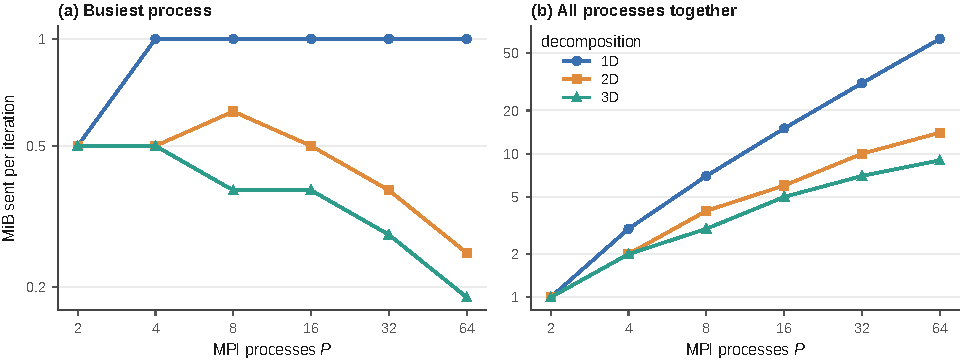
\includegraphics[width=\linewidth]{commvol}
\caption{Halo data sent per CG iteration for slab (1D), pencil (2D) and block (3D) decompositions,
$N=\CVN$, measured by the solver's counters. (a) The busiest process, which sets the exchange time on a
bandwidth-limited network; (b) the total network load.}\label{fig:commvol}
\end{figure}

\subsection{Halo exchange}\label{sec:halo}
Before each stencil application a process needs the values of the neighbouring blocks adjacent to its
faces. Because the 7-point stencil uses no edge or corner neighbours, the three directions are
independent and are exchanged together. In the \emph{blocking} mode the solver packs all six faces into
buffers within one OpenMP parallel region, performs one \code{MPI\_Sendrecv} per direction and sense,
unpacks the received faces into the ghost layers and then applies the stencil to the whole block.
Neighbours that do not exist are \code{MPI\_PROC\_NULL}, which turns the corresponding transfers into
no-ops.

The \emph{overlapped} mode exploits the fact that most points of a block do not need ghost values. It
posts \code{MPI\_Irecv} for all faces, packs, posts \code{MPI\_Isend}, applies the stencil to the interior,
waits for the messages, unpacks and finally applies the stencil to the remaining boundary shell. The shell
is covered by disjoint pieces---two $i$-planes, two $j$-rows inside them, two $k$-columns inside those---so
the fused inner product counts every point exactly once. Making this overlap effective took two further
steps. The first concerns progress: most MPI libraries move data only inside MPI calls, and large faces
use a rendezvous protocol, in which the data move only after a handshake with the matching receive, and
that handshake cannot complete while the process computes. The solver therefore
splits the interior sweep into chunks of $i$-planes (four by default) and calls \code{MPI\_Testall}
between them, which advances the transfers during the computation. The second concerns locality. Our first
version deferred the shell layers on all six sides, so with slabs every process handled its $k=1$ and
$k=n_z$ columns as isolated, strided points even though these lie on the physical boundary and need no
communication, which made the overlapped mode slower than the blocking one.
Restricting the deferred shell to layers that face an actual neighbour removed this penalty; what remains
is the cost of the second pass over the shell, which pays off only when messages take longer than that
pass (\cref{sec:variants}).

\subsection{Global reductions and three formulations of CG}\label{sec:reductions}
Classic CG (\cref{alg:cg}) performs two \code{MPI\_Allreduce} operations per iteration on a single value
each. Nothing useful can run while they are in flight, and with recursive doubling each costs about
$\lceil\log_2P\rceil$ network latencies. Two algebraically equivalent reformulations attack this term.

The Chronopoulos--Gear variant~[2] (\code{-a cg1}) introduces the auxiliary vectors $\vb w_k=A\vb r_k$ and
$\vb s_k=A\vb p_k$. Since $\vb p_k=\vb r_k+\beta_k\vb p_{k-1}$, linearity gives the recurrence
$\vb s_k=\vb w_k+\beta_k\vb s_{k-1}$, and the only stencil application per iteration becomes $\vb w_k=A\vb
r_k$. The denominator $\vb p_k^TA\vb p_k$ of the step length then follows from the two inner products
$\gamma_k=\vb r_k^T\vb r_k$ and $\delta_k=\vb w_k^T\vb r_k$ of the current iteration. Expanding
$\vb p_k=\vb r_k+\beta_k\vb p_{k-1}$ and using the CG identities $\vb r_k^TA\vb p_{k-1}=-\gamma_k/\alpha_{k-1}$
(orthogonality of successive residuals) and $\vb p_{k-1}^TA\vb p_{k-1}=\gamma_{k-1}/\alpha_{k-1}$ (definition
of $\alpha_{k-1}$) gives
\begin{equation}\label{eq:cg1}
  \vb p_k^TA\vb p_k=\delta_k-\frac{2\beta_k\gamma_k}{\alpha_{k-1}}+\frac{\beta_k^2\gamma_{k-1}}{\alpha_{k-1}}
  =\delta_k-\frac{\beta_k\gamma_k}{\alpha_{k-1}},\qquad
  \beta_k=\frac{\gamma_k}{\gamma_{k-1}},\qquad
  \alpha_k=\frac{\gamma_k}{\delta_k-\beta_k\gamma_k/\alpha_{k-1}} .
\end{equation}
Both inner products are now available at the same moment and travel in one \code{MPI\_Allreduce} of two
values. The four vector updates ($\vb p,\vb s,\vb x,\vb r$) and $\gamma$ are fused into one sweep and
$\delta$ into the stencil sweep, so the memory traffic per iteration stays that of classic CG.

The pipelined variant of Ghysels and Vanroose~[3] (\code{-a pipecg}) goes one step further and removes the
dependency between the reduction and the stencil. It adds $\vb z_k=A\vb s_k$ and $\vb q_k=A\vb w_k$ with
the recurrences $\vb z_k=\vb q_k+\beta_k\vb z_{k-1}$ and $\vb w_{k+1}=\vb w_k-\alpha_k\vb z_k$. Now
$\gamma_k$ and $\delta_k$ depend only on $\vb r_k$ and $\vb w_k$, which are known before $\vb q_k$ is
computed. The solver therefore starts an \code{MPI\_Iallreduce} of $(\gamma_k,\delta_k)$, computes $\vb
q_k=A\vb w_k$ while the reduction is in flight (polling it between stencil chunks, as for the halo), waits
for the result, evaluates \eqref{eq:cg1} and performs the six vector recurrences in one fused sweep that
also produces the next local $\gamma$ and $\delta$. The reduction latency disappears behind the stencil.
The price is three extra vectors, 36\% more memory traffic, and recurrences for $\vb w$ and $\vb z$ whose
rounding errors are never corrected, which limits the attainable accuracy (\cref{sec:validation}).

\subsection{Threads within a process}\label{sec:threads}
MPI is initialised with \code{MPI\_THREAD\_FUNNELED}: only the master thread calls MPI, always outside
parallel regions. Every loop nest is an \code{omp parallel for collapse(2) schedule(static)} over the
$(i,j)$ index pairs with an \code{omp simd} loop over the contiguous $k$ index, and the fused inner
products are OpenMP reductions. Arrays are 64-byte aligned and initialised with the same static schedule
that later computes on them, so on multi-socket nodes the first-touch policy (Linux places a page in the memory
of the socket that first writes it) puts each thread's pages in its own NUMA domain, the memory attached to
its socket. Processes and threads are pinned (\code{-{}-map-by ppr:$n$:node:PE=$T$
-{}-bind-to core}, \code{OMP\_PLACES=cores}, \code{OMP\_PROC\_BIND=close}), so the threads of one process
share a socket. Fewer processes with more threads reduce the number of messages, the number of reduction
participants and the ghost memory; in exchange every kernel pays a fork--join, the start and the closing barrier
of an OpenMP parallel region (five parallel regions per
iteration with blocking halos, up to about fifteen with overlap), and the worker threads idle while the
master thread waits in MPI.

\subsection{Offloading to GPUs}\label{sec:gpu-design}
The GPU solver (\code{src/cg\_gpu.c}) keeps the decomposition and the MPI structure of the CPU code and
replaces the threads of each process by one GPU: OpenMP is used for target offload, the ``X'' of
MPI\,+\,X. Processes on a node take consecutive devices (\code{omp\_set\_default\_device} on the node-local
rank). All vectors are allocated in GPU memory once, with \code{omp target enter data}, and never leave it
during the solve, because a single transfer of one vector over PCIe would cost more than a whole iteration
on the device. Every kernel---stencil with fused inner product, fused vector updates, face packing and
unpacking---is an \code{omp target teams distribute parallel for collapse(3)} loop over data that is
already present, and inner products are OpenMP reductions on the device followed by \code{MPI\_Allreduce}
on the host. The halo exchange packs each face on the GPU, copies only the packed faces to host buffers
(\code{omp target update}), exchanges them with \code{MPI\_Sendrecv} and copies them back for unpacking, so
the bus carries $V$ values per iteration instead of whole vectors. Classic CG and CG1 are available. Every
kernel is launched once before the clock starts, so the one-off kernel loading of the CUDA runtime is not
charged to the iteration.

\subsection{Performance model}\label{sec:model}
The decisions above enter the time per iteration through four terms,
\begin{equation}\label{eq:model}
  t_{\text{iter}}(P)\;\approx\;\frac{N^3}{P}\,\frac{B_v}{b(P)}\;+\;m\,t_s+V\,t_w\;+\;\rho\,\lceil\log_2P\rceil\,t_s ,
\end{equation}
where $B_v$ is the memory traffic per grid point of the CG variant (\cref{tab:variants-cost}), $b(P)$ the
memory bandwidth available to one process when $P$ processes share the hardware, $m$ and $V$ the message
count and halo volume of the busiest process from \eqref{eq:volume}, $t_s$ the latency of a message,
$t_w$ the transfer time per value, and $\rho$ the number of reductions per iteration that are not hidden.
$B_v$ counts explicit loads and stores in the convention of the STREAM benchmark~[5], which measures the
sustainable memory bandwidth with simple vector kernels, assuming that the
stencil's neighbour values are reused from cache. For classic CG the stencil reads $\vb p$ and writes $\vb
q$, the $\vb x,\vb r$ update reads four vectors and writes two, and the $\vb p$ update reads two and writes
one: $2+6+3=11$ accesses, or 88 bytes. Fusing the two inner products into these sweeps avoids three further
reads. On a CPU the stencil's pure write of $\vb q$ first loads the cache line (\emph{write-allocate}), which
adds 8 bytes; we therefore convert times into DRAM bandwidth with 96 bytes per point on the CPU and 88 on
the GPU, whose caches write full sectors without reading them.

\begin{table}[t]
\centering\small
\caption{Cost of the three CG formulations per iteration.}\label{tab:variants-cost}
\begin{tabular}{lcccc}
\toprule
variant & reductions $\rho$ & values each & vectors & $B_v$ (B/point) \\
\midrule
classic CG & 2 & 1 & 4 & 88 \\
Chronopoulos--Gear (CG1) & 1 & 2 & 5 & 88 \\
pipelined CG & 0 (overlapped) & 2 & 7 & 120 \\
\bottomrule
\end{tabular}
\end{table}

The model makes the scaling behaviour explicit. The memory term falls like $1/P$ only while $b(P)$ stays
constant, that is, until the processes on a socket saturate its memory bandwidth; from then on adding
cores on the same socket gains nothing, while adding nodes adds bandwidth. The halo term falls like
$P^{-2/3}$ for blocks and not at all for slabs. The reduction term grows with $\log_2P$ and is the only
term that grows, so it eventually dominates every strong-scaling run. CG1 halves it at no cost in $B_v$,
and pipelined CG removes it at a 36\% higher $B_v$, which pays off once the hidden latency exceeds the extra
memory time.

\section{Validation}\label{sec:validation}

We validate the solvers at three levels: agreement with the serial code, convergence to the exact
solution, and attainable accuracy. The script \code{scripts/validate.sh full} runs all CPU tests and
\code{scripts/check\_validation.py} evaluates them; \code{scripts/run\_gpu.sh} repeats the first level on
the GPU. All tests pass.

The first level compares every parallel configuration with the serial solver point by point. We ran all
combinations of the three CG variants, the two halo modes and the three decompositions on
$P\in\{1,2,3,4,6,8\}$ processes with $T\in\{1,2\}$ threads ($T=2$ for $P\le4$) on a $\ValN^3$ grid, chosen
because $40$ is not divisible by 3 or 6 so that uneven blocks occur. Each run writes its solution in
global order with collective MPI-IO (\code{MPI\_Type\_create\_subarray} and \code{MPI\_File\_write\_all}),
and the file is compared with the serial solution. \Cref{tab:validation} summarises the \ValRuns{} runs.
Classic CG and CG1 agree with the serial code to \ValWorstCG{} relative to the solution's maximum, which is
rounding level and stems only from the different summation order of the distributed inner products, and
they need exactly the serial number of iterations (\ValIters). Pipelined CG agrees to \ValWorstPipe{}, the
effect of its extra recurrences and still seven orders of magnitude below the discretisation error
(\ValErrMax). A further \ValEdge{} runs cover the corner cases of the shell decomposition of
\cref{sec:halo}---one-plane slabs, two-point blocks, $N=7$ on six processes and $N=2$ on two---and all
reproduce the serial solution to rounding level. On Vanda the quick suite (\NodeValRuns{} variant runs,
\NodeValEdge{} edge cases and the grid study) ran on a 32-core \NodeCPU{} node and \NodeValResult{} with
the same worst differences, \NodeValCG{} and \NodeValPipe. The GPU solver ran CG and CG1 on $P=\GpuValP$
processes sharing one A40, so that the $P=8$ runs exchange halos in all three directions through device
packing, host staging and MPI; all \GpuValRuns{} runs need 146 iterations and agree with the serial solution
to \GpuValWorst.

The 2D problem passes the same tests. \ValTwoRuns{} parallel runs on a $100^2$ grid (100 is not divisible
by 3, three CG variants, two halo modes, slabs and 2D blocks, $P=1$ to $8$, $T=1,2$) reproduce the serial
2D solution to \ValTwoWorstCG{} with classic CG and CG1 and to \ValTwoWorstPipe{} with pipelined CG, all
in the serial \ValTwoIters{} iterations; \ValTwoEdge{} corner cases down to $N=2$ agree to rounding level,
and the GPU solver agrees to \GpuValTwoWorst{} on $P=\GpuValTwoP$ processes.

\begin{table}[htb]
\centering\small
\caption{Parallel against serial solution on the $\ValN^3$ (3D) and $100^2$ (2D) grids. ``max diff'' is
$\max|x_{\text{par}}-x_{\text{ser}}|/\max|x_{\text{ser}}|$ over all runs of a row; ``true residual'' is the
largest $\|\vb b-A\vb x\|/\|\vb b\|$ at tolerance $\varepsilon=10^{-8}$.}\label{tab:validation}
\begin{tabular}{lllrcccrr}
\toprule
problem & algorithm & halo & runs & $P$ & $T$ & iterations & max diff & true residual \\
\midrule
\tabinput{generated/tab_validation.tex}
\bottomrule
\end{tabular}
\end{table}

The second level checks that the solver computes the solution of the differential equation and not only
of some linear system. \Cref{tab:convergence} and \cref{fig:validation}(a) report the discrete $L^2$ error
$\|u_h-u\|_{L^2}=\bigl(h^3\sum_{ijk}(u_{ijk}-u(x_i,y_j,z_k))^2\bigr)^{1/2}$ for $N=16$ to $128$, solved to
$\varepsilon=10^{-10}$ so that the algebraic error is negligible. The observed order is $\OrderMin$ to $\OrderMax$,
the order of the 7-point scheme, and $\OrderTwoMin$ to $\OrderTwoMax$ for the 5-point scheme on
$N=\ConvTwoNmin$ to $\ConvTwoNmax$ in 2D, and the parallel errors match the serial ones in every printed digit.

\begin{table}[htb]
\centering\small
\caption{Grid convergence of the serial solver and of the parallel solver ($P=4$, blocks, overlapped halo).}\label{tab:convergence}
\begin{tabular}{rcrccc}
\toprule
$N$ & $h$ & iterations & $\|u_h-u\|_{L^2}$ serial & $\|u_h-u\|_{L^2}$ parallel & observed order \\
\midrule
\tabinput{generated/tab_convergence.tex}
\bottomrule
\end{tabular}
\end{table}

The third level probes the numerical price of the reformulations. \Cref{fig:validation}(b) runs the three
variants towards a tolerance of $10^{-15}$ and records both the recursively updated residual, which the
algorithm sees, and the true residual $\|\vb b-A\vb x_k\|$, computed with an extra untimed stencil
application. CG and CG1 are indistinguishable, and their true residual levels off at \FloorCG{} once
rounding errors in $\vb x$ dominate. Pipelined CG follows them until the two residuals separate near
\SplitPipe; its best true residual is \FloorPipe, \FloorRatio{} times worse than CG, and when the iteration
continues its recursive residual stagnates while the true residual drifts back up, to as much as
\DriftPipe{} within \LastPipe{} iterations. This is the residual gap of pipelined Krylov methods: latency hiding costs
numerical robustness. On the $\ValN^3$ validation grid all three variants still meet $\varepsilon=10^{-8}$
(\cref{tab:validation}), but the gap grows with the problem: on the $\NS^3$ grid of \cref{sec:solve} the
true residual of pipelined CG ends at \SolvePipeRatio{} times the tolerance its recursive residual reports.
Production use of the pipelined variant therefore needs residual replacement, i.e.\ periodically
recomputing $\vb r=\vb b-A\vb x$ and $\vb w=A\vb r$ explicitly.

\begin{figure}[t]
\centering
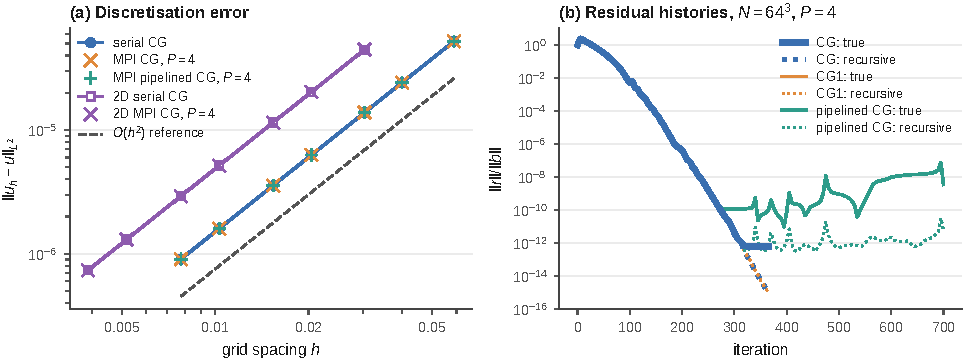
\includegraphics[width=\linewidth]{validation}
\caption{(a) Discretisation error against grid spacing for the serial and parallel solvers in 3D and 2D,
with an $O(h^2)$ reference line. (b) True (solid) and recursively updated (dotted) relative residuals,
$N=64$, $P=4$; the CG and CG1 curves coincide.}\label{fig:validation}
\end{figure}

\section{Performance}\label{sec:perf}

\paragraph{Setup.}
All measurements were taken on the NUS Vanda cluster through PBS Pro. The nodes we used carry two
\MachineCPU{} processors with \MachineCPS{} cores each and two NUMA domains. The multi-node job
requested \MachineNodes{} chunks of \MachineCPN{} cores on \MachineNodes{} different nodes, and on every node
PBS assigned the same \MachineCPN{} cores, the odd-numbered cores 9--71, which Linux numbers on the second
socket of these nodes. Each node thus contributes one socket and its memory controllers, and the job is a
clean model of a cluster of \MachineCPN-core nodes. MPI processes on remote
nodes were started through PBS (\code{pbs\_tmrsh}), which keeps them inside the job's CPU set (the cores PBS assigned to the job), and every
process was pinned to its own core. The code was built with GCC \MachineGCC{} (\code{-O3 -march=native
-fopenmp}) and run with \MachineMPI. Strong scaling keeps the global problem fixed while $P$ grows; weak scaling keeps the problem
per process fixed and enlarges the global grid with $P$. Strong-scaling runs use $N=\NS$ (\NSdofs{}
million unknowns, four to seven vectors of 1.07\,GB each) and $N=\NStwo$ (\NStwoDofs{} million
unknowns) in 3D and $N=\TwoN$ (\TwoDofs{} million unknowns) in 2D; weak-scaling runs use
$\WeakLocal^3$ and $\TwoWeakLocal^2$ points per process. Each timing run performs exactly \Iters{} iterations of the steady-state
loop; work vectors are allocated before the clock starts, and the one-off setup stencil application of CG1
and pipelined CG counts in the time to solution but not in the time per iteration. Every configuration ran
\Reps{} times, interleaved with the others (the complete solves of \cref{sec:solve} once), and we report the fastest run (median spread
\MedSpread\% in 3D, 3.3\% in 2D); the $256\times1$ split of \cref{sec:hybrid} is the same configuration as strong scaling at
$P=256$, and the two sets of runs are pooled. The GPU runs used one \GpuName{} (48\,GB, driver \GpuDriver) on a Vanda GPU node,
compiled with \code{nvc} \GpuNVC{} of the NVIDIA HPC SDK (\code{-O3 -mp=gpu -gpu=cc86}).

\subsection{Serial baseline and problem size}\label{sec:serial}

\Cref{fig:sizes} and \cref{tab:sizes} run the serial solver on one core for $N=\SzNmin$ to $\SzNmax$, so
the matrix dimension grows from $0.26$ to $134$ million and the number of nonzeros from $1.8$ to $938$
million. The time per iteration grows like $N^{\SzSlopeIter}$, i.e.\ linearly in the number of unknowns, as
expected for a matrix-free method whose every kernel is a sweep over the vectors. The cost per grid point
stays between \SzNsMin{} and \SzNsMax\,ns over the whole range, with no step where the four vectors (\SzMiBSmall\,MiB
at $N=\SzNmin$, \SzGiBLarge\,GiB at $N=\SzNmax$) outgrow the 67.5\,MiB L3 cache of a socket near $N=128$: one core draws
\SzBwMin--\SzBwMax\,GB/s whether the data comes from L3 or from DRAM, because its bandwidth is limited by
the number of cache misses it can keep in flight, not by the memory level (\cref{sec:strong}). The
iteration count grows linearly in $N$, from \SzItMin{} to \SzItMax{} iterations ($\SzItPerNmin\,N$ to $\SzItPerNmax\,N$),
so the time to solution grows like $N^{\SzSlopeSolve}$ and reaches \SzSolveMax\,s, \SzSolveMaxMin{}
minutes, on the $512^3$ grid. Doubling the resolution from 256 to 512 makes the solve \SzDoubling{} times more expensive,
close to the factor 16 of the $N^4$ law; this is the work that the parallel solver has to distribute. The
serial baseline for all speedups below, \SerialTiter\,ms per $512^3$ iteration, comes from the single-node
job \code{pbs/vanda\_node.pbs} on the same processor type.

The 2D solver covers $N=\SzTwoNmin$ to $\SzTwoNmax$, from 0.07 to \SzTwoDofsMax{} million unknowns and
from 0.33 to 336 million nonzeros (\cref{tab:sizes2d}). Its cost per grid point shows the cache step that
the 3D runs did not: at $N=\SzTwoNmin$ the touched part of the four vectors, about 2\,MiB, fits into the core's
private 2\,MiB L2 cache and an update costs \SzTwoNsSmall\,ns, from $N=\SzTwoNsecond$ to 1024 the data come from
L3 (\SzTwoNsSecond\,ns), and from 2048 on from DRAM, where the cost reaches \SzTwoNsLarge\,ns at $8192^2$, or
\SzTwoBwLarge\,GB/s against \SzBwLarge\,GB/s in 3D. The iteration count again grows linearly in $N$, $\SzTwoItPerNmin\,N$
to $\SzTwoItPerNmax\,N$, so the 2D time to solution grows like $N^{\SzTwoSlopeSolve}$, between the $N^3$ of
the ideal law and the cache effects at the small end, and reaches \SzTwoSolveMax\,s for $N=\SzTwoNsolveMax$.

\begin{figure}[t]
\centering
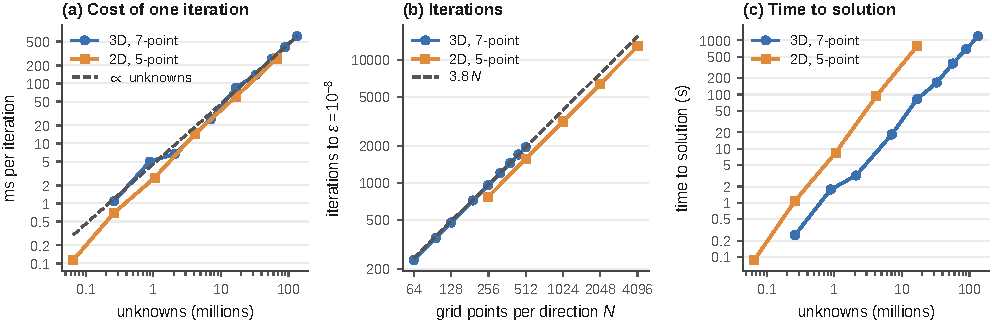
\includegraphics[width=\linewidth]{sizes}
\caption{Serial solver on one core of an \SizesCPU{} node, 3D and 2D problem. (a) Time per iteration
against the matrix dimension; (b) iterations to $\varepsilon=10^{-8}$; (c) time to solution against the
matrix dimension. Dashed lines: cost proportional to the number of unknowns and iterations proportional to
$N$.}\label{fig:sizes}
\end{figure}

\begin{table}[t]
\centering\small
\caption{Serial problem-size study: unknowns and nonzeros (millions), memory of the four vectors with ghost layers (MiB),
time per iteration (best of three 20-iteration runs and the complete solve), cost per grid point, effective DRAM bandwidth (96
B/point), iterations and time to $\varepsilon=10^{-8}$, and the maximum error against the exact
solution.}\label{tab:sizes}
\begin{tabular}{rrrrrrrrrc}
\toprule
$N$ & unknowns & nonzeros & MiB & ms/iter & ns/point & GB/s & iterations & solve (s) & max error \\
\midrule
\tabinput{generated/tab_sizes.tex}
\bottomrule
\end{tabular}
\end{table}

\begin{table}[t]
\centering\small
\caption{Serial problem-size study of the 2D problem, columns as in \cref{tab:sizes} (the 2D grid is
stored with three $j$-planes, so the MiB column is three times the touched data). Complete solves up to
$N=\SzTwoNsolveMax$.}\label{tab:sizes2d}
\begin{tabular}{rrrrrrrrrc}
\toprule
$N$ & unknowns & nonzeros & MiB & ms/iter & ns/point & GB/s & iterations & solve (s) & max error \\
\midrule
\tabinput{generated/tab_sizes2d.tex}
\bottomrule
\end{tabular}
\end{table}

\subsection{Strong scaling from one core to \NodesMax{} nodes}\label{sec:strong}

\Cref{fig:strong} and \cref{tab:strong} show the baseline configuration: pure MPI, blocks, overlapped halo
and classic CG, \MachineCPN{} processes per node. The parallel code on one process is \PoneVsSerial\%
\PoneFaster{} than the serial code, so the parallel machinery costs nothing. The curve has two regimes
separated by the node boundary.

Inside one socket the speedup is ideal up to four processes (\SpeedupFour, \EffFour\% efficiency) and then
flattens: \SpeedupEight{} on eight processes and \SpeedupNode{} on 32, an efficiency of \EffNode\%.
Communication does not explain this, because halo exchange and reductions take \CommFracNode\% of the
iteration at $P=32$. \Cref{fig:bandwidth} converts the time per iteration into DRAM traffic with the
96-byte model of \cref{sec:model} and compares it with the STREAM triad counted the same way. One core
moves \CGbwOne\,GB/s, more than single-threaded STREAM (\StreamOne\,GB/s): the solver's
six-vector update keeps more independent memory streams in flight than the three of the triad. Both grow almost linearly to eight
cores (\CGbwEight{} and \StreamEight\,GB/s). Beyond that the solver flattens, \CGbwSixteen\,GB/s on 16
cores and \CGbwNode\,GB/s on 32, \CGbwFrac\% of the socket's STREAM bandwidth (\StreamAll\,GB/s), which
keeps climbing. Cores added after the memory controllers
saturate have nothing to compute on: inside a socket the speedup of CG is the bandwidth speedup.

Across nodes the picture reverses, because every node adds a socket's worth of memory bandwidth. Going
from one node to two cuts the iteration from \TiterNode{} to \TiterSixtyFour\,ms (\NodeEffSixtyFour\% node-level
efficiency), and \NodesMax{} nodes reach \TiterPmax\,ms, \NodeSpeedPmax{} times faster than one node
(\NodeEffPmax\% efficiency) and \SpeedupPmax{} times faster than the serial code. The aggregate traffic
rises to \CGbwAll\,GB/s, \CGbwTB\,TB/s: \CGbwFracNodes\% of eight times what the solver draws on one node,
and \CGbwFracStreamNodes\% of the dotted line in \cref{fig:bandwidth}, eight times the STREAM bandwidth of a
socket. On the larger $\NStwo^3$ grid, where each process
owns 3.4 times more points but sends only 2.25 times more halo data, \NodesMax{} nodes are \NodeSpeedTwoPmax{} times faster
than one (\TiterTwoNode{} to \TiterTwoPmax\,ms), \NodeEffTwoPmax\% efficiency. The efficiency that is lost
across nodes is lost to communication, which \cref{sec:comm} dissects.

\begin{figure}[t]
\centering
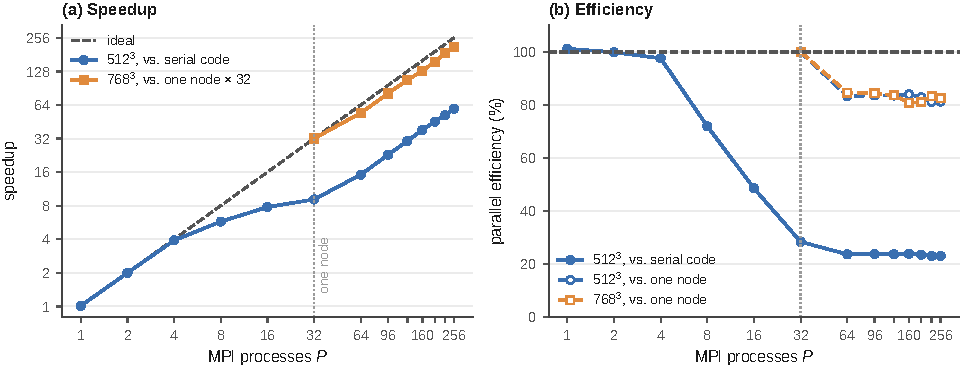
\includegraphics[width=\linewidth]{strong}
\caption{Strong scaling of the baseline (pure MPI, 3D blocks, overlapped halo, classic CG), 32 processes
per node. $512^3$: speedup and efficiency relative to the serial code (solid) and relative to one node
(dashed, $32\,t_{32}/(P\,t_P)$); $768^3$: relative to one node.}\label{fig:strong}
\end{figure}

\begin{table}[t]
\centering\small\setlength{\tabcolsep}{4.5pt}
\caption{Strong scaling, \Iters{} iterations. ``eff'' is $S(P)/P$ relative to the serial code, ``node eff''
relative to one node; ``comm'' is the share of the iteration spent in halo exchange and reductions,
including waiting; ``halo'' is the data sent by the busiest process per iteration.}\label{tab:strong}
\begin{tabular}{rrcrrrrrrrr}
\toprule
 & & & \multicolumn{6}{c}{$N=\NS^3$} & \multicolumn{2}{c}{$N=\NStwo^3$}\\
\cmidrule(lr){4-9}\cmidrule(lr){10-11}
$P$ & nodes & process grid & ms/iter & speedup & eff (\%) & node eff (\%) & comm (\%) & halo (KiB) & ms/iter & node eff (\%) \\
\midrule
\tabinput{generated/tab_strong.tex}
\bottomrule
\end{tabular}
\end{table}

\begin{figure}[t]
\centering
\begin{minipage}[t]{0.49\linewidth}\centering
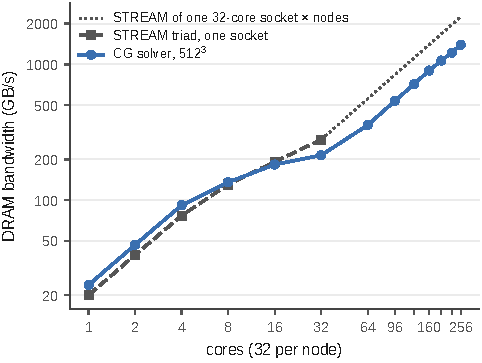
\includegraphics[width=\linewidth]{bandwidth}
\caption{DRAM traffic of the $512^3$ baseline (96 bytes per point and iteration) against the STREAM triad
of one socket (32 bytes per element); the dotted line multiplies the socket's STREAM bandwidth by the
number of nodes.}\label{fig:bandwidth}
\end{minipage}\hfill
\begin{minipage}[t]{0.49\linewidth}\centering
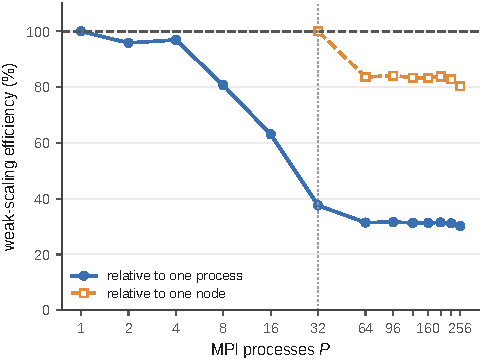
\includegraphics[width=\linewidth]{weak}
\caption{Weak scaling with $\approx\WeakLocal^3$ points per process: time per grid point and iteration
relative to one process and relative to one full node.}\label{fig:weak}
\end{minipage}
\end{figure}

\subsection{Where the communication time goes}\label{sec:comm}

The breakdown in \cref{fig:breakdown} splits each iteration into its four phases. On one process the
vector updates take \VecFracSerial\% of the time, more than the stencil, because they account for nine of
the eleven memory accesses per point while doing almost no arithmetic. Inside the node the communication
phases stay thin. Beyond it they grow with every node, and at $P=\Pmax$ they take \CommFracPmax\% of the
iteration.

The two kinds of communication behave very differently. The halo exchange is cheap: at $P=\Pmax$ the
busiest process sends \HaloKiBPmax\,KiB per iteration in six messages, which the network delivers in a few
tens of microseconds, and the whole phase, including face packing and unpacking, costs \HaloMsPmax\,ms or
\HaloFracPmax\% of the iteration. The reductions are expensive: they take \RedMsPmax\,ms, \RedFracPmax\%
of the iteration, although the two \code{MPI\_Allreduce} calls move 16 bytes and a reduction over 256
processes needs only about $\lceil\log_2 256\rceil=8$ network latencies, a few tens of microseconds. The
rest is waiting. Every process has the same amount of work (the $8\times8\times4$ process grid divides
$512^3$ evenly), but every process also shares its socket's memory bandwidth with 31 others and its node
with other jobs, so in each iteration some process finishes its sweep late, and the reduction makes all
\Pmax{} processes wait for it. On one node this barrier effect costs \RedMsNode\,ms per iteration; across
\NodesMax{} nodes, where the slowest of eight sockets sets the pace, it costs \RedMsPmax\,ms. The global
reductions, not the halo messages, are what limits strong scaling across nodes, and they act as barriers
far more than as messages. The model \eqref{eq:model} charges a reduction only its latency; on a real
machine the term that decides is the spread of the per-process sweep times, which every reduction exposes.

Weak scaling (\cref{fig:weak}) separates the two regimes. With \WeakLocal$^3$ points per process
one process completes an iteration in \WeakTone\,ms, drawing \WeakBwOne\,GB/s. Thirty-two processes on one
socket need \WeakTnode\,ms for 32 times the data, because they share the bandwidth (\WeakBwNode\,GB/s each);
the efficiency relative to one process falls to \WeakEffNode\%, the bandwidth wall again. From one node to
\WeakPmax{} processes on \NodesMax{} nodes, where each node brings its own memory, the time grows only from
\WeakTnode{} to \WeakTmax\,ms while the problem grows to $\WeakNmax^3$, \WeakDofsMax{} billion unknowns: a
node-level weak-scaling efficiency of \WeakNodeEff\%. Most of the loss occurs in the first step across the
network: two nodes need \WeakTtwo\,ms, and from three to seven nodes the time stays between \WeakTmidMin{}
and \WeakTmidMax\,ms, and eight nodes need \WeakTmax\,ms. Weak scaling of the time per iteration also flatters the algorithm: the iteration
count grows like $N\propto P^{1/3}$, so the time to solution grows by the same factor even when every
iteration scales perfectly, a growth that only a better preconditioner removes.

\begin{figure}[t]
\centering
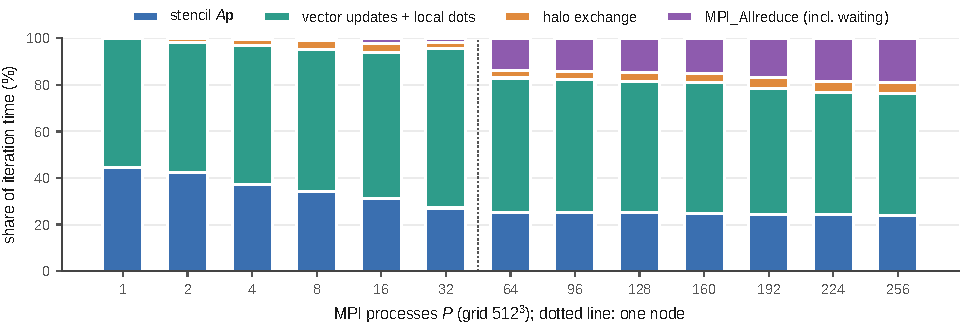
\includegraphics[width=\linewidth]{breakdown}
\caption{Share of the iteration time spent in the stencil, the vector updates, the halo exchange and the
reductions (each phase timed as the maximum over processes; the reduction time includes waiting for slower
processes; absolute times in \cref{tab:strong}).}\label{fig:breakdown}
\end{figure}

\subsection{Effect of the design choices across nodes}\label{sec:variants}

\Cref{fig:variants} and \cref{tab:variants} vary one decision at a time around the baseline on one to
\NodesMax{} nodes and report the time per iteration relative to the baseline at the same $P$.

The decomposition matters most, and the volume model of \cref{eq:volume} predicts it. Slabs are
\RelOneDmin{} times slower than blocks on one node and \RelOneD{} times slower on \NodesMax{} nodes: every
slab process ships two full $512^2$ planes, 4\,MiB per iteration whatever $P$, and at $P=256$ each slab is
only two planes thick, so a process sends as much data as it owns. Pencils are 1--6\% faster than blocks up to
224 processes, where their $P^{-1/2}$ halo volume is still close to the $P^{-2/3}$ of blocks and they avoid
the strided $k$-faces, and fall behind at $P=\Pmax$ (\RelTwoD).

Overlapping the halo exchange does not pay, even across the network. The blocking exchange runs at
\RelBlockingRange{} times the baseline, never measurably slower, and \RelBlocking{} on \NodesMax{} nodes. The reason is
the one found in \cref{sec:comm}: the messages are small and the network fast, so there is little transfer
time to hide, while the overlapped mode pays for the chunked interior sweep, the polling and the second pass
over the boundary shell. Overlap would pay with larger faces per process or a slower network.

The CG formulations confirm that the reduction time is waiting, not latency. CG1 merges the two
reductions into one and runs at \RelCGoneRange{} times classic CG at every process count (\RelCGonemin{} on
one node, \RelCGone{} on \NodesMax{}): a single barrier per iteration still has to wait for the slowest
process, and that process is no faster. Pipelined CG pays its traffic surcharge almost in full on one node
(\RelPipemin; the model predicts $128/96=1.33$ with write-allocate), and its relative cost falls to
\RelPipe{} on \NodesMax{} nodes, where more reduction time is there to hide. It does not break even:
the \code{MPI\_Iallreduce} hides the latency of the reduction behind the stencil, but not the waiting for
the slowest process, whose contribution still arrives late. On the larger $\NStwo^3$ grid, with less communication per byte of memory traffic, pipelined CG
remains \RelPipeTwo{} times slower on \NodesMax{} nodes.

\begin{figure}[t]
\centering
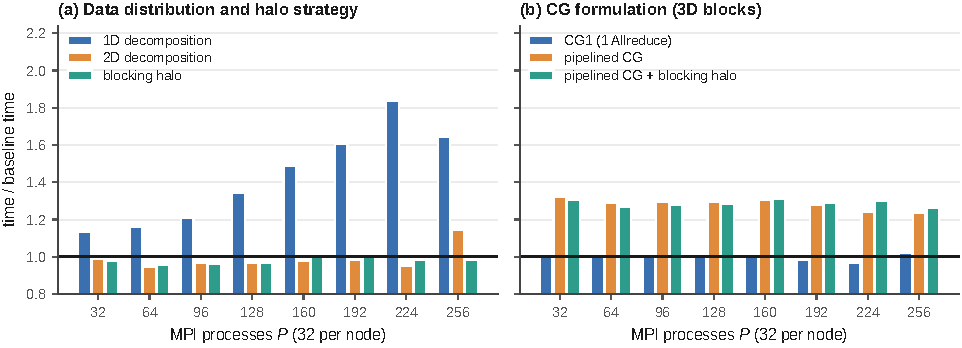
\includegraphics[width=\linewidth]{variants}
\caption{Time per iteration of each variant divided by the baseline (3D blocks, overlapped halo, classic CG)
at the same $P$, $N=\NS^3$, 32 processes per node; values below 1 are faster.}\label{fig:variants}
\end{figure}

\begin{table}[t]
\centering\small
\caption{Time per iteration in ms and, in parentheses, relative to the baseline; $N=\NS^3$, one, two, four
and eight nodes (\cref{fig:variants} shows all process counts).}\label{tab:variants}
\tabinput{generated/tab_variants_head.tex}
\tabinput{generated/tab_variants.tex}
\bottomrule
\end{tabular}
\end{table}

\subsection{Processes versus threads on \HybCores{} cores}\label{sec:hybrid}

\Cref{fig:hybrid} and \cref{tab:hybrid} keep all \HybCores{} cores busy and vary the split into MPI
processes and OpenMP threads, from 256 single-threaded processes to eight processes with 32 threads, one
per node. All splits lie within \HybRange\% of each other, so the hybrid code loses nothing to its threads.
The best split is \HybBest{} (\HybBestT\,ms), \HybGain\% faster than pure MPI (\HybPureT\,ms): four
processes per socket mean eight times fewer participants in each reduction and fewer, larger halo
messages, and the reduction wait drops from \HybRedPure{} to \HybRedBest\,ms per iteration. With more
threads per process the fork--join cost of the many parallel regions per iteration grows, and one process
per node with 32 threads (\HybWorstT\,ms) ties with \HybSecond{} (\HybSecondT\,ms) as the slowest split. The right
configuration is four processes per socket with eight threads each.

\begin{figure}[t]
\centering
\begin{minipage}[t]{0.46\linewidth}\centering\vspace{0pt}
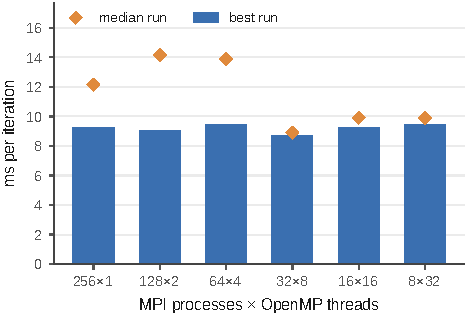
\includegraphics[width=\linewidth]{hybrid}
\caption{Time per iteration for different process $\times$ thread splits of the same 256 cores, $512^3$.}\label{fig:hybrid}
\end{minipage}\hfill
\begin{minipage}[t]{0.5\linewidth}\centering\small\vspace{0pt}
\captionof{table}{Process $\times$ thread splits on 256 cores: best and median time per iteration and the
halo and reduction parts of the best run (ms, including waiting).}\label{tab:hybrid}
\begin{tabular}{rrrrrr}
\toprule
$P$ & $T$ & best & median & halo & reduce \\
\midrule
\tabinput{generated/tab_hybrid.tex}
\bottomrule
\end{tabular}
\end{minipage}
\end{figure}

\subsection{The 2D problem}\label{sec:twod}

\Cref{fig:twod} and \cref{tab:strong2d} repeat the scaling study for the 2D problem on the same eight
nodes: $\TwoN^2$ for strong scaling, $\TwoWeakLocal^2$ points per process for weak scaling, 2D blocks,
overlapped halo and classic CG as the baseline. Inside a socket the 2D solver hits the same bandwidth
wall: one process needs \TwoPoneT\,ms per iteration, 32 processes \TwoTnode\,ms, a speedup of
\TwoSpeedNode{} at \TwoBwNode\,GB/s. Across nodes it scales better than the 3D solver. Eight nodes reach
\TwoTmax\,ms, \TwoNodeSpeedMax{} times faster than one node, \TwoNodeEffMax\% efficiency against
\NodeEffPmax\% in 3D, and \TwoSpeedMax{} times faster than one process. Both problems end at the same
aggregate traffic on eight nodes, \TwoBwMax{} and \CGbwAll\,GB/s. The weak-scaling runs show the same
picture: one node is at \TwoWeakEffNode\% of the single-process rate, and from one to eight nodes the
time per iteration only grows from \TwoWeakTnode{} to \TwoWeakTmax\,ms while the grid grows to
$\TwoWeakNmax^2$, \TwoWeakDofsMax{} billion unknowns, a node-level weak-scaling efficiency of
\TwoWeakNodeEff\% against \WeakNodeEff\% in 3D.

The communication budget explains the difference. A process of the $\TwoN^2$ run on 256 cores owns a
\TwoLocalMax{} block and sends \TwoHaloKiBMax\,KiB per iteration in \TwoMsgsMax{} messages, twenty times
less than in 3D, and the halo phase costs \TwoHaloMsMax\,ms, \TwoHaloFracMax\% of the iteration. The
reductions cost \TwoRedMsMax\,ms, \TwoRedFracMax\% of it: the barrier wait of \cref{sec:comm} is a
property of the global synchronisation of CG and appears in both problems, while the halo cost is a property of the
geometry and vanishes in 2D.

The geometry also reverses the decomposition result. In 2D, slabs are faster than blocks at every process
count, \TwoSlabMin{} times the baseline on one node and \TwoSlabMax{} on eight. A slab process sends two
contiguous rows of $\TwoN$ values, \TwoSlabHaloKiB\,KiB per iteration in two messages, which the network
delivers in microseconds, and in return it saves the strided $k$-faces and the extra messages of the
blocks and sweeps rows sixteen times longer. The halo-to-owned ratio $2P/N$ of \cref{sec:decomp} stays at a
few percent in 2D, whereas in 3D the slab halo equals the slab, so the decomposition that has to be avoided
in 3D is the one to use in 2D. The other two choices behave as in 3D: the blocking halo runs at
\TwoBlockRange{} times the baseline, and CG1 at \TwoCGoneRange, \TwoCGoneMax{} on eight nodes. The
complete solve on 256 cores needs \TwoSolveIters{} iterations; it takes \TwoSolveCG\,s with classic CG,
\TwoSolveSpeedup{} times faster than one process, and \TwoSolveCGone\,s with CG1, a \TwoSolveCGoneGain\%
gain against 2\% in 3D.

\begin{figure}[t]
\centering
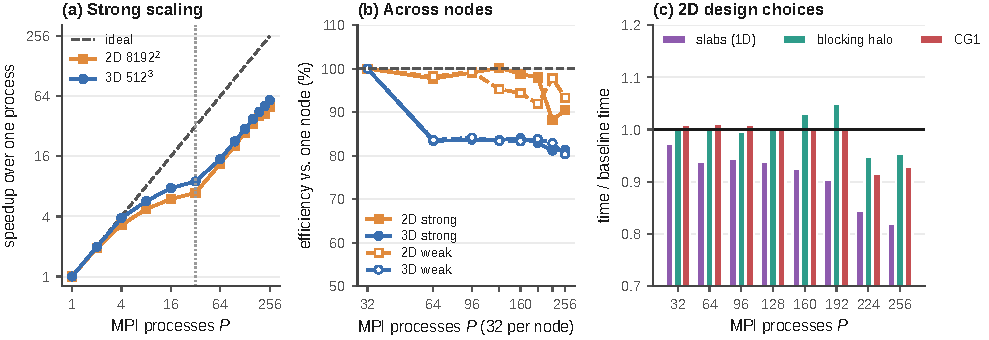
\includegraphics[width=\linewidth]{twod}
\caption{The 2D problem on 1 to 256 processes, 32 per node. (a) Strong-scaling speedup over one process,
$\TwoN^2$ against $512^3$; (b) efficiency relative to one node of strong ($32\,t_{32}/(P\,t_P)$) and weak
scaling for both problems; (c) time per iteration of slabs, blocking halo and CG1 divided by the 2D
baseline (2D blocks, overlapped halo, classic CG).}\label{fig:twod}
\end{figure}

\begin{table}[t]
\centering\small\setlength{\tabcolsep}{4.5pt}
\caption{2D strong scaling ($N=\TwoN^2$, \Iters{} iterations) and weak scaling ($\TwoWeakLocal^2$ points
per process). ``eff'' is relative to one process, ``node eff'' relative to one node; ``comm'' is the share of
the iteration spent in halo exchange and reductions; ``halo'' is the data sent by the busiest process per
iteration.}\label{tab:strong2d}
\begin{tabular}{rrcrrrrrrrr}
\toprule
 & & & \multicolumn{6}{c}{strong, $N=\TwoN^2$} & \multicolumn{2}{c}{weak}\\
\cmidrule(lr){4-9}\cmidrule(lr){10-11}
$P$ & nodes & process grid & ms/iter & speedup & eff (\%) & node eff (\%) & comm (\%) & halo (KiB) & ms/iter & node eff (\%) \\
\midrule
\tabinput{generated/tab_strong2d.tex}
\bottomrule
\end{tabular}
\end{table}

\subsection{GPU offload}\label{sec:gpu}

\Cref{fig:gpu} and \cref{tab:gpu} run the offload solver on one A40 from $N=\GpuNmin$ to $N=\GpuNmax$,
the largest grid holding \GpuDofsMax{} million unknowns. Above $128^3$ the GPU sustains a constant
\GpuBwAboveMin--\GpuBwMax\,GB/s of DRAM traffic, \GpuBwFrac\% of its nominal 696\,GB/s; at $128^3$
(\GpuBwMin\,GB/s) the grid is too small to fill the device and the launch overhead of the three kernels per
iteration shows. The two vector-update kernels stream at \GpuVecBw\,GB/s, \GpuVecBwFrac\% of the peak. The
stencil takes \GpuSpmvFrac\% of an iteration and reaches only \GpuSpmvBw\,GB/s of compulsory traffic
(read $\vb p$, write $\vb q$), \GpuSpmvBwFrac\% of the peak: its neighbour values from the adjacent planes are
not all reused from the GPU's small caches and are fetched from memory more than once. CG1 is \GpuCGoneRel\% slower than classic CG on the GPU: its fused five-vector
kernel saves no traffic, and there are no reductions to merge on a single device.

On the $512^3$ grid one A40 needs \GpuTfiveTwelve\,ms per iteration and moves \GpuBwFiveTwelve\,GB/s. That
is \GpuVsSocket{} times faster than a 32-core CPU socket, \GpuVsCore{} times faster than one core and
\GpuVsEight{} times slower than the \NodesMax{} nodes of \cref{sec:strong}; the time ratio to the socket is the
ratio of the bandwidths the two sustain (\GpuBwFiveTwelve{} against \CGbwNode\,GB/s, \GpuBwRatio) times the
factor $96/88$ the GPU saves by not reading lines before writing them. The 2D problem runs at the same bandwidth: from $\GpuTwoNmin^2$ to
$\GpuTwoNmax^2$ (\GpuTwoDofsMax{} million unknowns) the A40 sustains \GpuTwoBwMin--\GpuTwoBwMax\,GB/s,
and the $\GpuTwoN^2$ iteration takes \GpuTwoT\,ms (\GpuTwoBw\,GB/s), \GpuTwoVsSocket{} times faster than
a CPU socket and \GpuTwoVsEight{} times slower than eight nodes. Its 5-point stencil reaches
\GpuTwoSpmvBw\,GB/s, more than the 7-point stencil, because it has no neighbours in other planes to fetch
twice. With several GPUs every halo message passes
through host memory twice; a CUDA-aware MPI would send the packed faces directly from device memory and
remove both copies.

\begin{figure}[t]
\centering
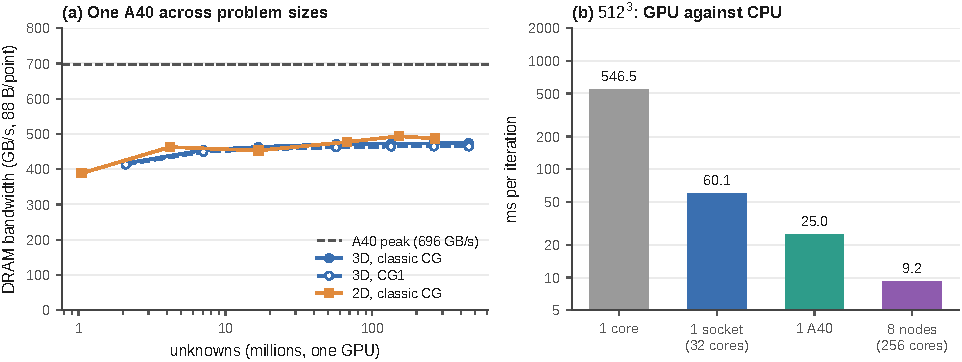
\includegraphics[width=\linewidth]{gpu}
\caption{(a) DRAM bandwidth of the offload solver on one NVIDIA A40 for the 3D and 2D problems (88 bytes
per point and iteration).
(b) Time per iteration on the $512^3$ grid: serial code, one 32-core socket, one A40 and eight nodes.}\label{fig:gpu}
\end{figure}

\begin{table}[t]
\centering\small
\caption{One A40: unknowns (millions), memory of the four CG vectors (GiB), time per iteration of classic CG
and CG1 (best of 3 runs of 50 iterations), DRAM bandwidth, share of the stencil kernel, and billions of
grid-point updates per second.}\label{tab:gpu}
\begin{tabular}{rrrrrrrr}
\toprule
$N$ & unknowns & GiB & CG ms/iter & CG1 ms/iter & GB/s & stencil (\%) & GLUP/s \\
\midrule
\tabinput{generated/tab_gpu.tex}
\midrule
\multicolumn{8}{l}{2D problem ($N^2$ grid; GiB include the two unused ghost planes)} \\
\tabinput{generated/tab_gpu2d.tex}
\bottomrule
\end{tabular}
\end{table}

\subsection{Time to solution}\label{sec:solve}

\Cref{tab:solve} closes the loop with complete solves of the $512^3$ problem to $\varepsilon=10^{-8}$. All
runs stop after \SolveIters{} iterations and reach the same error against the exact solution, which at this
tolerance is set by the discretisation. At the serial baseline rate the serial code
needs $\SolveIters\times\SerialTiter$\,ms $=\SolveSerialEst$\,s. \Pmax{} cores on \NodesMax{} nodes solve the problem in
\SolveCG\,s with classic CG and \SolveCGone\,s with CG1, \SolveSpeedup{} times faster; one A40 needs
\SolveGpu\,s. Pipelined CG takes \SolvePipe\,s and is the only
variant whose answer is worse: its true residual ends at \SolvePipeTrue, \SolvePipeRatio{} times the
tolerance its recursive residual reports. The residual gap of \cref{sec:validation} grows with the problem
and is the second cost of hiding the reduction, next to the extra memory traffic. The 2D solves need
\TwoSolveIters{} iterations; 256 cores take \TwoSolveCG\,s and one A40 \GpuTwoSolve\,s. After that many
iterations the true residual of classic CG ends at \TwoSolveTrue, and the error against the exact
solution sits at the discretisation level.

\begin{table}[t]
\centering\small
\caption{Complete solves to $\varepsilon=10^{-8}$ of the $\NS^3$ and $\TwoN^2$ problems (CPU runs: 3D or 2D
blocks, overlapped halo, 32 processes per node). ``speedup'' is relative to the serial baseline rate, $\SolveIters\times\SerialTiter$\,ms
$=\SolveSerialEst$\,s, for 3D and relative to the
one-process rate, $\TwoSolveIters\times\TwoPoneT$\,ms $=\TwoSolveSerialEst$\,s, for 2D.}\label{tab:solve}
\setlength{\tabcolsep}{4pt}
\begin{tabular}{lllrrrccr}
\toprule
problem & platform & algorithm & iterations & time (s) & ms/iter & true residual & max error & speedup \\
\midrule
\tabinput{generated/tab_solve.tex}
\bottomrule
\end{tabular}
\end{table}

\section{Conclusions}\label{sec:conclusion}

We built a matrix-free Conjugate Gradient solver for the 2D and 3D Poisson equation in a serial, a hybrid
MPI\,+\,OpenMP and an MPI\,+\,OpenMP offload version, in which decomposition, halo exchange, reduction
strategy and threading are run-time switches. All versions reproduce the serial solution to rounding level
and converge to the exact solution at the theoretical second order, so every performance difference we
measure is a property of the parallel design.

The problem is parallelised by distributing the grid in 3D blocks with one ghost layer, so that each
process applies the stencil to its own block after a six-message halo exchange, and by turning each inner
product into a local OpenMP or GPU reduction followed by a global \code{MPI\_Allreduce}. Its performance is
set by memory bandwidth first and by the reductions second. Inside a socket the solver scales exactly as
far as the memory controllers do, \CGbwFrac\% of STREAM on 32 cores and a speedup of \SpeedupNode. Across
nodes each socket adds bandwidth, and \Pmax{} cores on \NodesMax{} nodes reach a speedup of \SpeedupPmax{}
over the serial code, \NodeEffPmax\% strong-scaling efficiency relative to one node on $512^3$,
\NodeEffTwoPmax\% on $768^3$ and \WeakNodeEff\% weak-scaling efficiency on 1.8 billion unknowns.

The part of the algorithm that communicates most in time is not the part that communicates most in bytes.
The halo exchange moves all of the data---\HaloKiBPmax\,KiB per process and iteration at $P=\Pmax$---and
costs \HaloFracPmax\% of the iteration; the two reductions move 16 bytes and cost \RedFracPmax\%, because
every reduction is a barrier at which \Pmax{} processes wait for the slowest one. The design choices follow
from this. Blocks are the decomposition to use: slabs send as much as they compute and run \RelOneD{}
times slower on \NodesMax{} nodes, and pencils fall \RelTwoD{} times behind at $P=\Pmax$. Overlapping the halo exchange hides little and is at most 1\% faster than the
blocking exchange. Merging the two reductions (CG1) costs nothing but gains nothing measurable, because the
time at the barrier is waiting, not latency. Pipelining the reduction hides its latency but not the
waiting, adds a third more memory traffic and degrades the true residual \SolvePipeRatio-fold, so it does
not pay on this machine. The lever that remains is load balance: anything that makes every process finish
its sweep at the same moment shortens every barrier. A few MPI processes per socket with eight OpenMP
threads each cut the reduction wait and give the fastest split on \HybCores{} cores. One A40 GPU runs an
iteration \GpuVsSocket{} times faster than a CPU socket and solves the $512^3$ problem in \SolveGpu\,s.

The 2D problem separates the two mechanisms. Its halo nearly disappears, the barrier wait at the
reductions remains, and eight nodes reach \TwoNodeEffMax\% strong and \TwoWeakNodeEff\% weak efficiency
relative to one node. It also shows that the right decomposition depends on the geometry: slabs, the
worst choice in 3D, are the best one in 2D.

The next steps follow from the same analysis: a multigrid or Chebyshev preconditioner, which removes the
$O(N)$ growth of the iteration count, and communication-avoiding $s$-step methods, which perform one
reduction per $s$ iterations and attack the barrier cost directly.

\paragraph{Code and data.} The source code, the PBS job scripts, the scripts that produce every figure and
table, the raw CSV measurements and job logs, and a \code{README.md} with full run instructions are open
source (MIT licence) at \url{https://github.com/davidzuo023/dsa5208-project3} [7].

\paragraph{Use of AI tools.} We used Claude (Anthropic) as a coding and writing assistant. Under our
direction it wrote most of the implementation, the test and benchmark scripts and a first draft of this
report. We chose the problem and the parallelisation questions, obtained access to Vanda and ran all jobs
there, checked the results against the validation suite, and reviewed and edited the report. All numbers
in this report come from our runs; the commit history of the repository reflects this workflow.

\section*{References}
\begin{enumerate}\footnotesize\setlength{\itemsep}{0pt}\setlength{\parsep}{0pt}
\item M.~R.~Hestenes and E.~Stiefel. Methods of conjugate gradients for solving linear systems.
\emph{J.\ Res.\ Nat.\ Bur.\ Standards} 49:409--436, 1952.
\item A.~T.~Chronopoulos and C.~W.~Gear. $s$-step iterative methods for symmetric linear systems.
\emph{J.\ Comput.\ Appl.\ Math.} 25:153--168, 1989.
\item P.~Ghysels and W.~Vanroose. Hiding global synchronization latency in the preconditioned Conjugate
Gradient algorithm. \emph{Parallel Computing} 40:224--238, 2014.
\item J.~Dongarra, M.~A.~Heroux and P.~Luszczek. High-performance conjugate-gradient benchmark: a new metric
for ranking high-performance computing systems. \emph{Int.\ J.\ High Perform.\ Comput.\ Appl.}
30(1):3--10, 2016.
\item J.~D.~McCalpin. Memory bandwidth and machine balance in current high performance computers.
\emph{IEEE TCCA Newsletter}, 1995.
\item J.~R.~Shewchuk. \emph{An Introduction to the Conjugate Gradient Method Without the Agonizing Pain}.
Carnegie Mellon University, 1994.
\item Y.~Wu, D.~Zuo and C.~Zhu. \emph{dsa5208-project3: Conjugate Gradients for the 3D Poisson equation with
MPI, OpenMP and GPU offload}. Source code, 2026. \url{https://github.com/davidzuo023/dsa5208-project3}.
\end{enumerate}

\end{document}
